%- HandOut Flag -----------------------------------------------------------------------------------------
\makeatletter
\@ifundefined{ifHandout}{%
  \expandafter\newif\csname ifHandout\endcsname
}{}
\makeatother

%- D0cum3nt ----------------------------------------------------------------------------------------------
\documentclass[beamer,10pt]{standalone}   
%\documentclass[beamer,10pt,handout]{standalone}  \Handouttrue  

\ifHandout
	\setbeameroption{show notes} %print notes   
\fi

	
%- Packages ----------------------------------------------------------------------------------------------
\usepackage{custom-style}
\usetikzlibrary{positioning}
\usepackage{multicol}


%--Beamer Style-----------------------------------------------------------------------------------------------
\usetheme{toninus}
\usepackage{animate}
\usetikzlibrary{positioning, arrows}
\usetikzlibrary{shapes}

\begin{document}

%------------------------------------------------------------------------------------------------

% Frame inspired by Leonid: passing from moment maps to comoment maps
\begin{frame}[fragile]{Reminder: Moment maps in symplectic geometry}
	Let $(M,\omega)$ be a symplectic manifold, $\vartheta: G\times M \to M$ a Lie group action preserving $\omega$ and $v:\mathfrak{g}\to \mathfrak{X}(M)$ the corresponding infinitesimal action
	%
		\begin{defblock}[Moment map pertaining to $\vartheta$]
			Smooth map $ \mu: M \to \mathfrak{g}^\ast$ such that: \stackunder{$d \langle\mu , \xi \rangle = \iota_{v_\xi}\omega \scriptstyle\quad \forall \xi \in \mathfrak{g}$}{$f (\vartheta_g(x)) = Ad^\ast_g (f(x)) \scriptstyle\quad \forall g \in G, x \in M$}
		\end{defblock}
	%
	\vfill
	\emph{... from a dual perspective (assuming $G$ connected) ...}
			\begin{defblock}[Comoment map pertaining to $v$]
				\begin{columns}
					\begin{column}{.5\linewidth}	
			Lie algebra morphism \qquad $ f: \mathfrak{g} \to C^\infty(M) $
			\\
			such that \qquad $ d~f (x) = -\iota_{v_x} \omega \qquad \forall x \in \mathfrak{g}~.$
					\end{column}
					\begin{column}{.4\linewidth}	
						\begin{displaymath}
							\begin{tikzcd}
								& C^{\infty}(M,\omega) \ar[d]
								\\
								\mathfrak{g} \ar[ur,dashed,"(f)"]\ar[r,"v"']& \mathfrak{X}(M)
							\end{tikzcd}	
						\end{displaymath}
					\end{column}
				\end{columns}
		\end{defblock}		
	%
	\vfill
	\emph{... a tool encoding conserved quantities ...}
	\begin{propblock}[Noether Theorem]
		\small Fixed $H\in C^\infty_{\text{Ham}}(M)$ ($\mathfrak{g}$-invariant) ,
				$$\mathcal{L}_{v_H} f(x) = 0 \qquad \forall x \in \mathfrak{g}$$
	\end{propblock}
\end{frame}
%\note[itemize]{
%	\item comoment map is a Lie algebra morphism projecting to $v$. (Triangle diagram in Lie algebra category).
%}



%------------------------------------------------------------------------------------------------
\begin{frame}{Geometry of symmetries}\label{frame:geometrysymmetries}
	Basic mechanical structures are encoded in geometry. but there is another complementary geometrical property that's natural in physics: symmetry!
	\begin{alertblock}{Upshot}
		Continous symmetries are described by actions of a Lie group on $M$.
	\end{alertblock}
	\begin{block}{Noether}
		Presence of symmetries $\quad \Rightarrow \quad$ existence of conserved quantities.
	\end{block}	
	\begin{block}{Key concept:}
		Noether current are encoded in a \emph{moment map}  $\mu :M \rightarrow \mathfrak{g}^*$ (the dual of the comoment map $f$. 
	\end{block}
  \begin{columns}[T]
   	\begin{column}{.6\textwidth}
			\begin{block}{Symplectic reduction:}
			\begin{itemize}
				\item System dynamics should be restricted to level set of conserved observables in order to efficiently store dynamical properties.
				\item Under certain assumptions, $\mu^{-1}( 0 )/G$ is a symplectic manifold with an "induced" symplectic structure.
			\end{itemize}
			\end{block}
    \end{column}
    \begin{column}{.4\textwidth}	
			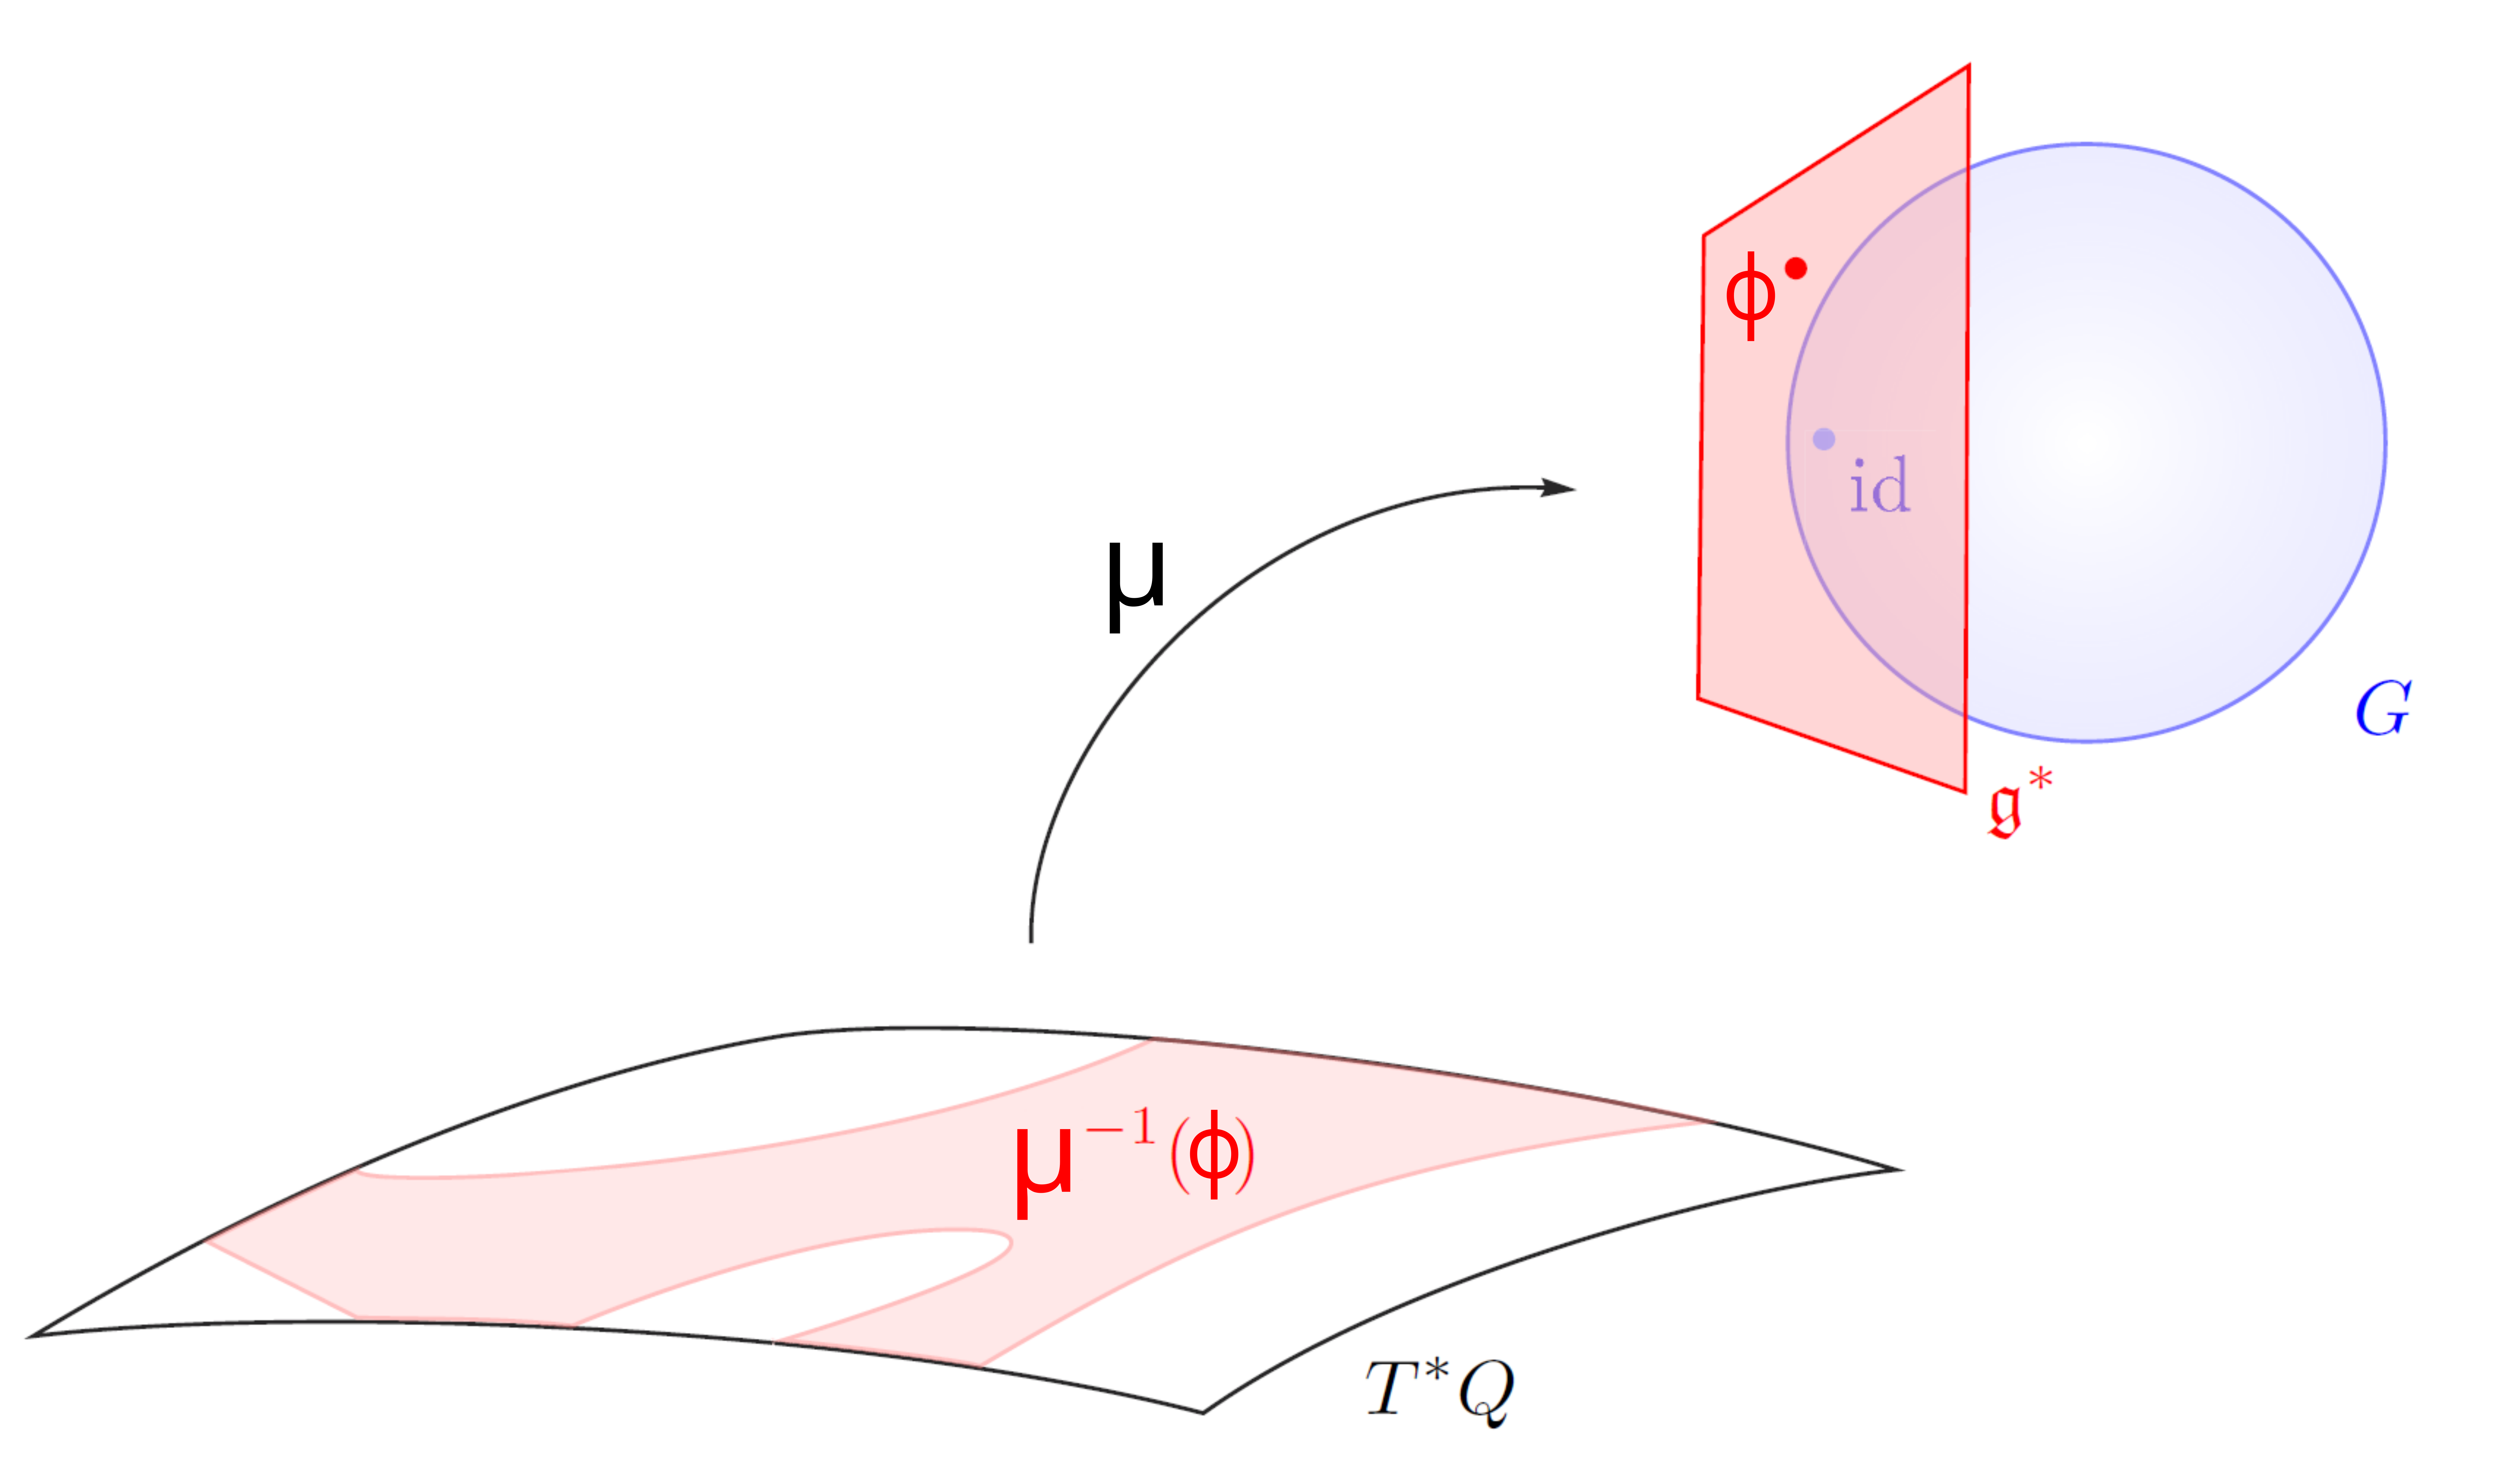
\includegraphics[width=\textwidth]{Pictures/Reduction} 
  	\end{column}
	\end{columns}			
\end{frame}
%------------------------------------------------------------------------------------------------



%---------------------------------------------------------------------------------------------------------------------------------------------------
\begin{frame}{Research proposal context: (multi)symplectic reduction}
	\textbf{\color{UniGreen}Symplectic reduction:}~~
	Procedure associating to any (suitably regular) pair of symplectic manifold and Hamiltonian action another symplectic manifold of smaller dimension.
	\vfill
	\pause
	\begin{thmblock}[Marsden-Weinstein reduction]
		\vspace{-.4em}
		\begin{tabular}{l p{12cm}}
		    Given: & $(M,\omega)$ symplectic
		    \\
		    & $G\curvearrowright M$ symplectic with equivariant momap. $J:M\to \mathfrak{g}^*$
		    \\[.2em]
		    Assume: & $\mu \in \mathfrak{g}^*$ regular value of $J$ 
		    \qquad\quad \footnotesize \textcolor{gray}{($\Rightarrow$ $J^{-1}(\mu)\hookrightarrow M$ smooth embedding)}
		    \\
			& $G_\mu\action J^{-1}(\mu)$ free and proper
			\quad \footnotesize \textcolor{gray}{($\Rightarrow$ $J^{-1}(\mu)/G_\mu$ smooth manifold)}
			\\[.4em]
			Then: & $\exists!$ symplectic structure $\omega_\mu$ in $M_\mu:= J^{-1}(\mu)/G_\mu$ \\
			& s.t. $\pi^\ast \omega_\mu = j^\ast \omega$ with $j:M_\mu \hookrightarrow M$ and $\pi:M\twoheadrightarrow M_\mu$
		\end{tabular}
		\vspace{-.4em}
	\end{thmblock}
	%
	\vfill
	\pause
	\begin{columns}
		\begin{column}{0.40\textwidth}
			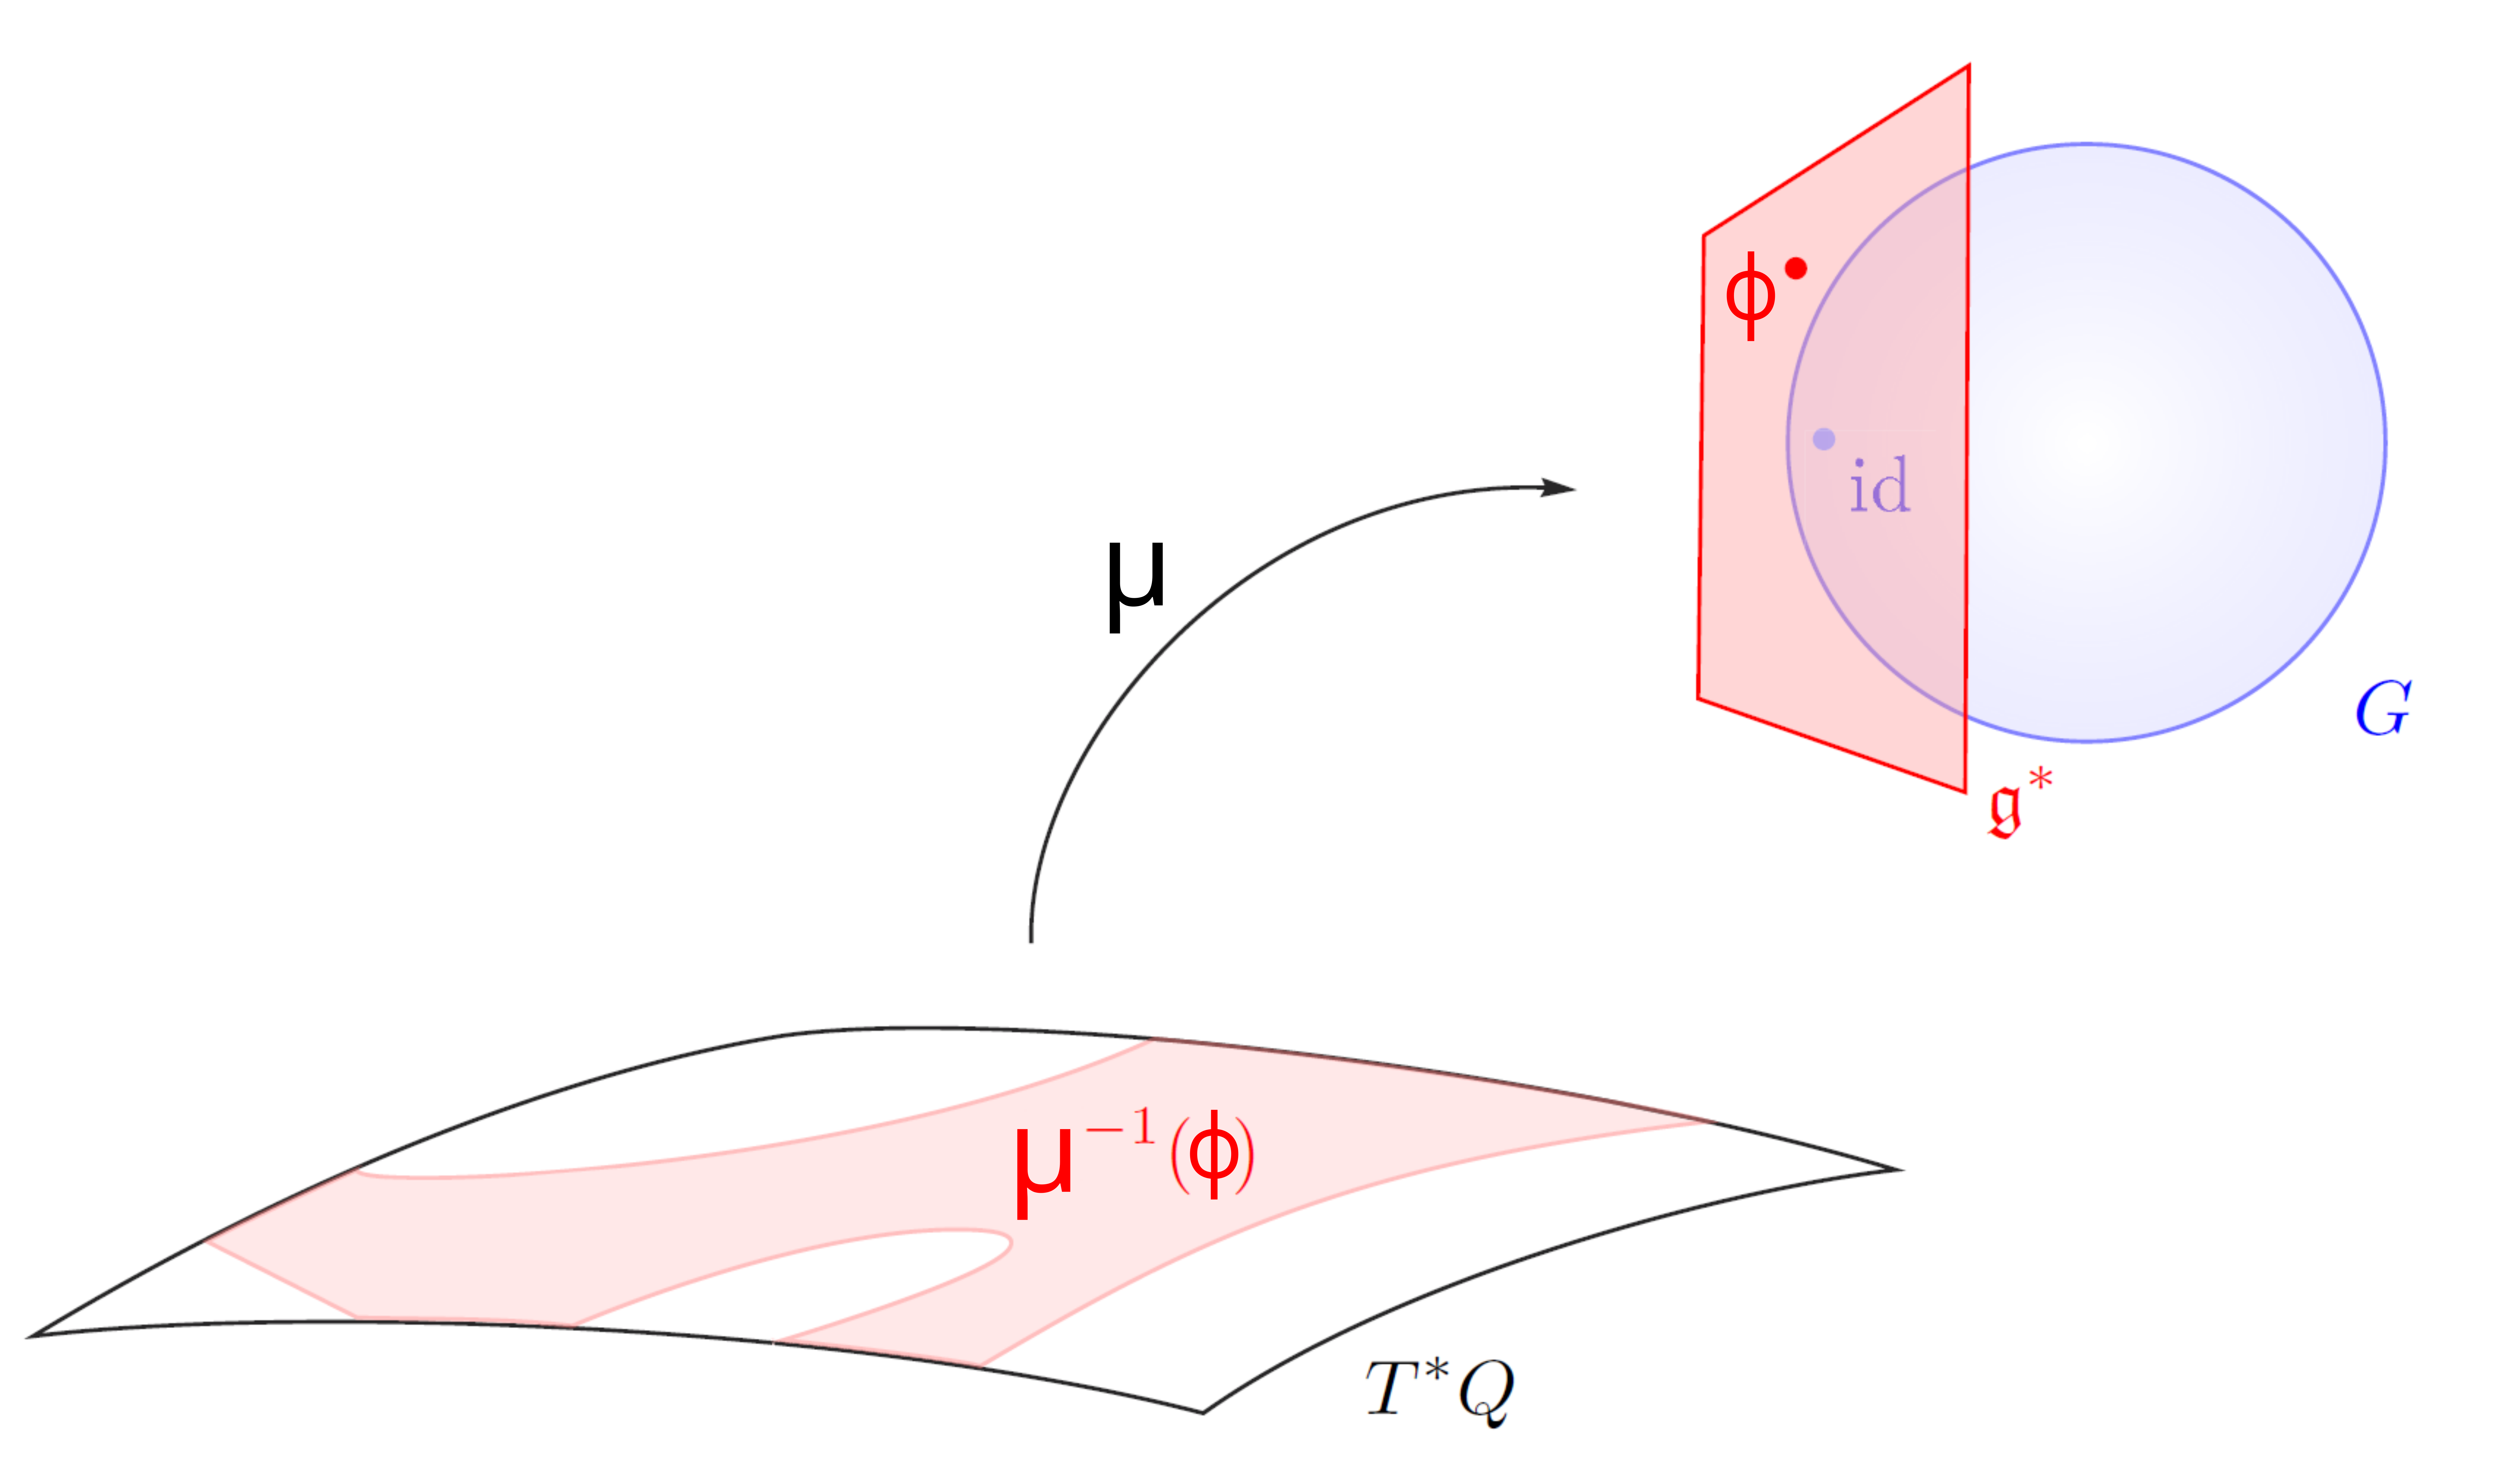
\includegraphics[width=\textwidth]{Pictures/Reduction}
		\end{column}	
		
		\begin{column}{0.6\textwidth}
				\textbf{\color{UniGreen}In mechanics:}~~
			it embodies the process of restricting the dynamics of the system to the level sets of the conserved quantities pertaining to the symmetry group.		
			\\
			\color{gray}\small( e.g. restricting to studying a point-like particle in a central potential by studying it in radial coordinates only)
		\end{column}	
	\end{columns}	


\end{frame}
%---------------------------------------------------------------------------------------------------------------------------------------------------

%-------------------------------------------------------------------------------------------------------------------------------------------------
\begin{frame}[fragile,shrink]{Homotopy co-moment maps \emph{(Callies, Fregier, Rogers, Zambon)}}
	\begin{columns}
		\begin{column}{.625\linewidth}	
			HCMM is an $L_\infty$-morphism  $\quad(f):\mathfrak{g}\to L_\infty(M,\omega)$
			\\[.5em]
			 lifting the  infinitesimal action $\quad v:\mathfrak{g}\to \mathfrak{X}(M)$
		\end{column}
		\begin{column}{.325\linewidth}	
			\begin{displaymath}
				\begin{tikzcd}[column sep = large]
					& L_{\infty}(M,\omega) \ar[d,"\mathscr{v}"]
					\\
					\mathfrak{g} \ar[ur,dashed,"(f)"]\ar[r,"v"']& \mathfrak{X}(M)
				\end{tikzcd}	
			\end{displaymath}		
		\end{column}
	\end{columns}
	\pause
	\begin{lemblock}[HCMM unfolded  \cite{Callies2016}]
			%
			HCMM is a sequence of (graded-skew) multilinear maps:
			\begin{displaymath}
				(f)  = \big\lbrace f_k: \; \Lambda^k{\mathfrak g} \to L_{k-1} \subseteq \Omega^{n-k} 
				\;\big\vert\; 0\leq k \leq n+1  \big\rbrace
			\end{displaymath}
			%
			\vspace{-.5em}	
			\includestandalone[width=0.9\textwidth]{Pictures/Frame_HCMM}
			
			\vspace{-1em}		
			\emph{fulfilling:}%\emph{such that:}
			\begin{itemize}
				\item<2-> $f_0 = 0 $, $f_{n+1} = 0$
				\item<3-> $d f_k (p) = f_{k-1} (\partial p)  - (-1)^{\frac{k(k+1)}{2}} \iota(v_p) \omega 
				\qquad\scriptstyle \forall p \in \Lambda^k(\mathfrak{g}),\; \forall k=1,\dots n+1$
			\end{itemize}
		\end{lemblock}

	\begin{tamblock}
	 Practically a HCMM is given by several multilinear maps
	 \begin{displaymath}
	 	f_i = \Lambda^i \mathfrak{g} \to L_{i-1}
	 \end{displaymath}
	 satisfying:
	 \begin{enumerate}
	 	\item $ d f_1(\xi) = - \iota_{v_\xi} \omega$
	 	\item $\sum ...$
	 \end{enumerate}
	\end{tamblock}


\end{frame}
\note[itemize]{
	%\item 		Consider:  $v:\mathfrak g\to \mathfrak X(M)$  a Lie algebra morphism  s.t. $\mathcal{L}_{v_x}\omega=0 \quad  \forall x\in\mathfrak g$ (i.e infinitesimal multisymplectic Lie algebra action $\mathfrak{g}\circlearrowleft (M,\omega)$)
	\item More conceptually, a comoment is an $L_\infty$-morphism $(f):\mathfrak{g}\to L_\infty(M,\omega)$ lifting the action $v:\mathfrak{g}\to \mathfrak{X}(M)$, 
i.e. making the diagram commute in the $L_\infty$-algebras category.
	\item The vertical arrow is the trivial $L_\infty$-extension of the function mapping any Hamiltonian form to the unique corresponding Hamiltonian vector field (an it is zero elsewhere)
		\\
		(Note that any Lie algebra can be seen as an $L_\infty$-algebra concentrated in degree $0$, therefore any $L_\infty$-morphism $L\to\mathfrak{g}$ is simply given by a linear map $L_0 \to \mathfrak{g}$ preserving the binary brackets.)
	\item We will make use of an explicit version of this definition which is expressed by the lemma.
	 Practically speaking, a HCMM is given by several multilinear maps ...
	 \item In the equation we have tacitly set $\Lambda^{-1}(M) = 0$
	 %\item Notation: \qquad $\partial =$ Chevalley-Eilenberg boundary operator.
	%\item Notice that a HCMM pertains to an "infinitesimal" action of ${\mathfrak g}$ on $M$ with ${\mathfrak g}$ being the Lie algebra of a generic Lie group $G$, acting on $M$ by $\omega$-preserving vector fields.
		\item (Notation) $ p = \xi_1 \wedge \xi_2 \wedge \dots \wedge \xi_k$, 
			then $v_p = v_1 \wedge v_2 \wedge \dots \wedge v_k$ 
			where $v_i \equiv v_{\xi_i}$ are the fundamental vector fields associated to the action $G \circlearrowright M$.
	%	\item (Notation) $\iota(v_p) \omega = \iota(v_k)\dots\iota(v_1) \omega$
	%	\item $\varsigma(k) := - (-1)^{\frac{k(k+1)}{2}}$ 
		\item (Notation) $(\iota^{k}_{\mathfrak{g}}\omega)(p):= \iota(v_p) \omega = \iota(v_k)\dots\iota(v_1) \omega$
		\item $\partial \equiv \partial_k:  \Lambda^{k} {\mathfrak g} \to \Lambda^{k-1} {\mathfrak g}$  is the usual Eilenberg-Chevalley complex boundary operator (see appendix, pag: \ref{frame:CE-complex});
%		\item The definition tells us that the {\it closed} forms
%			$$\mu_k := f_{k-1} (\partial p) +  \varsigma(k) \iota(v_p) \omega 	$$
%			must actually be {\it exact}, with potential $-f_k(p)$.  	
		\item The last equation tells us that an HCMM is not a chain complex morphism but is rather a chain complex homotopy between 0 and the multicontraction $\alpha=(\iota^{k}_{\mathfrak{g}}\omega)$ (see next slide).
		is a chain map by lemma 2.18 \cite{Ryvkin2016}).
}
%---------------------------------------------------------------------------------------------------------------------------------

%-------------------------------------------------------------------------------------------------------------------------------------------------
\begin{frame}[t]{Symmetries in \textbf{multisymplectic geometry}}
	Consider a Lie algebra action $v:\mathfrak{g} \to \mathfrak{X}(M)$  preserving the $n$-plectic form $\omega$,
	\vfill

	\vspace{-1em}
	\begin{columns}[T]
		\setlength{\belowdisplayskip}{5pt}
		\begin{column}{.50\linewidth}
			%
			\centering \it
			\onslide<2->{
				$-$ symplectic case $-$
				\begin{defblock}[Comoment map pertaining to $v$]
					Lie algebra morphism
					$$ f: \mathfrak{g} \to C^\infty(M) $$
					such that
					$$ d~f (x) = -\iota_{v_x} \omega \qquad \forall x \in \mathfrak{g}~.$$
				\end{defblock}
			}
		\end{column}	
		%
		\onslide<2->{\vrule{}}
		%
		\begin{column}{.50\linewidth}
			\centering \it
			\onslide<3->{			
				$-$ $n$-plectic case $-$
				\begin{defblock}[Homotopy comoment map \tiny (HCMM)]
					$L_\infty$-morphism 
					$$ (f_k) : \mathfrak{g} \to L_\infty (M,\omega)$$
					such that
					$$ d~f_1(x) = -\iota_{v_x} \omega \qquad \forall x \in \mathfrak{g}~.$$
				\end{defblock}	
			}
		\end{column}	
	\end{columns}	
	%
	\pause
	\vfill
	\centering 
	\onslide<4->{\textbf{-- Conserved quantities --}}
	%
	\vspace{-.5em}
	\begin{columns}[T]
		\setlength{\belowdisplayskip}{5pt}
		\begin{column}{.50\linewidth}
			%
			\centering \it
			\onslide<4->{
			\begin{propblock}[Noether Theorem]
				\small Fixed $H\in C^\infty_{\text{Ham}}(M)$ ($\mathfrak{g}$-invariant) ,
				$$\mathcal{L}_{v_H} f(x) = 0 \qquad \forall x \in \mathfrak{g}$$
			\end{propblock}
			}
		\end{column}	
		%
		\onslide<5->{\vrule{}}
		%
		\begin{column}{.50\linewidth}
			\centering \it
			\onslide<5->{			
			\begin{propblock}[RWZ16 Theorem]
				\small Fixed $H\in \Omega^{n-1}_{\text{Ham}}(M)$ ($\mathfrak{g}$-invariant),
				$$\mathcal{L}_{v_H} f_k(p) \in B^k(M) \qquad \forall p \in Z_k(\mathfrak{g})$$			
			\end{propblock}
			}
		\end{column}	
	\end{columns}		
\end{frame}
%-------------------------------------------------------------------------------------------------------------------------------------------------


\end{document}